% -------------------------------------------------------------------------
\section{Numerical experiments}\label{sec:experiments}
% -------------------------------------------------------------------------

We now evaluate the new version of lookout in five simulation experiments. Experiments 1 and 2 compare it against the original version, Experiments 3 to 5 compare both versions with four other anomaly detection methods, and \cref{sec:bwablation} examines the sensitivity of the results to the bandwidth. Two further comparisons of the two versions, a set of showcase examples, and the details of \cref{sec:bwablation} are in the online Appendix. Both versions are run in the current implementation, version 2.1.0 of the \texttt{lookout} package \citep{Rlookout}. 

The four other methods, also used for comparison by \citet{lookout}, are HDoutliers \citep{wilkinson2017visualizing} and \textit{stray} \citep{stray}, which apply extreme value theory to nearest-neighbour distances, and KDEOS \citep{Schubert2014} and RDOS \citep{Tang2017}, which are based on kernel density estimates. HDoutliers and stray are run with $\alpha=0.01$ (the default for stray), and KDEOS and RDOS with their default settings. Experiments 1 and 2 report the true and false positive rates of the two versions of lookout. HDoutliers and stray return labels, so in Experiments 3 to 5 we compare them with lookout by the Fmeasure and Gmean,
$$
  \text{Fmeasure} = \frac{2\,\text{Precision}\times\text{Recall}}{\text{Precision} + \text{Recall}},
  \qquad
  \text{Gmean} = \sqrt{\text{Sensitivity} \times \text{Specificity}},
$$
where Precision $= \text{TP}/(\text{TP} + \text{FP})$, Recall $=$ Sensitivity $= \text{TP}/(\text{TP} + \text{FN})$ and Specificity $= \text{TN}/(\text{TN} + \text{FP})$, with TP, FP, TN and FN the numbers of true positives, false positives, true negatives and false negatives. KDEOS and RDOS return anomaly scores, so we compare them with the scores $p_i$ of lookout by the area under the ROC curve (AUC), the curve of sensitivity against one minus specificity over all thresholds.

\subsection{Experiment 1: Different anomaly rates for Gamma distribution}

The non-anomalous observations have independent gamma coordinates in $\R^2$ with shape 2 and rate 2, and the anomalies independent gamma coordinates with shape 2 and rate $r \in \{0.1, 0.2, \ldots, 1\}$. Each replication has 500 non-anomalies and 10 anomalies, and there are 10 replications for each value of $r$.

\begin{figure}[!b]
  \centering
  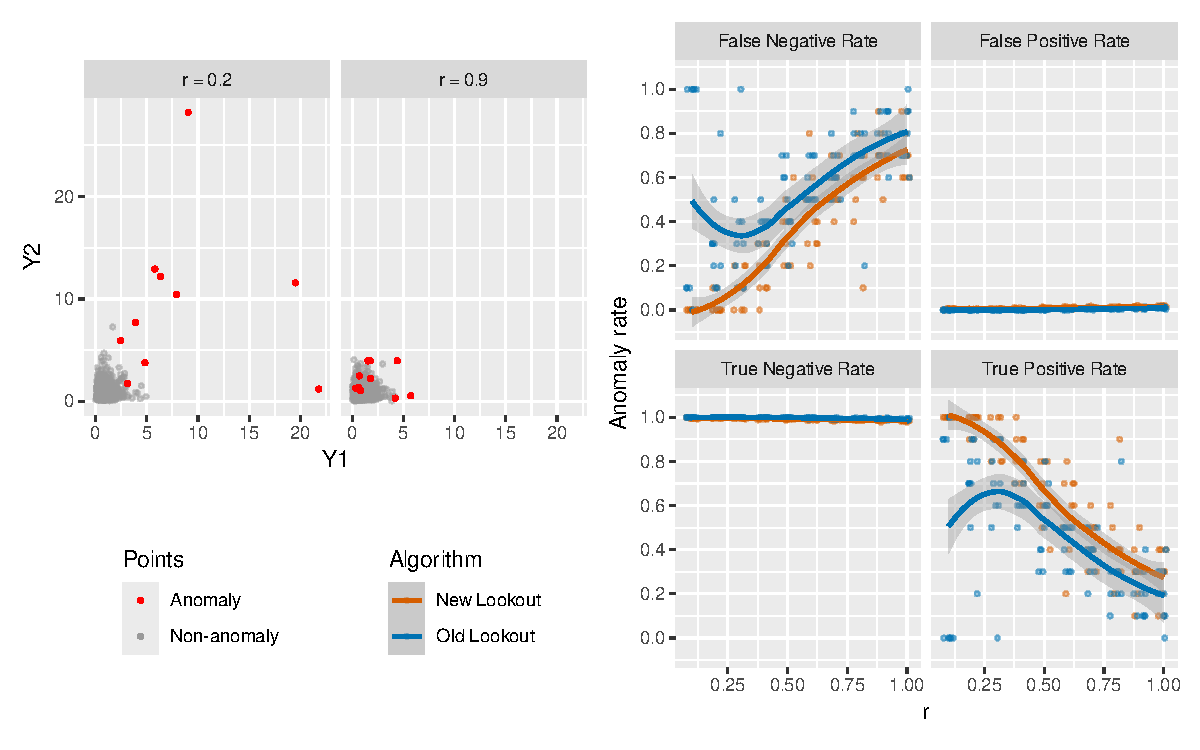
\includegraphics[width=\textwidth]{Figures/Exp1_Gamma_Rates.pdf}
  \caption{Experiment 1. Left: data with $r = 0.2$ and $r = 0.9$; anomalies with lower values of $r$ are easier to identify. Right: error rates of the two versions of lookout, with points jittered horizontally.}
  \label{fig:exp1}
\end{figure}

\cref{fig:exp1} shows the data and results. As $r$ increases the anomalies become more similar to the non-anomalies, so the true positive rate falls. The new version has a higher true positive rate than the original at every value of $r$ below 1, with the largest difference at $r=0.1$ (0.97 against 0.19), where the anomalies are farthest from the non-anomalous observations. Both versions have false positive rates of at most 0.012.

\subsection[Experiment 2: Anomalies on the boundary as n increases]{Experiment 2: Anomalies on the boundary as $n$ increases}

The non-anomalous observations have independent $\mathcal{N}(0,1)$ coordinates in $\R^2$, with $n \in \{1000, 2000, \ldots, 10000\}$, and there are $0.005n$ anomalies in a ring just beyond most of them. The anomaly means $\bm{\mu}_i$ lie on the circle of radius $2.2\sqrt2$ about the origin, with $\mu_{i1} \sim \mathcal{U}(-2.2\sqrt2, 2.2\sqrt2)$ and $\mu_{i2}$ negative for a randomly chosen half of the anomalies, and $Y_{ij} \sim \mathcal{N}(\mu_{ij}, 0.1^2)$ for $j=1,2$. There are 10 replications for each $n$, and for both versions the kernel density estimates use the truncated sum described in \cref{sec:modified}, with 100 neighbours.

\begin{figure}[!b]
  \centering
  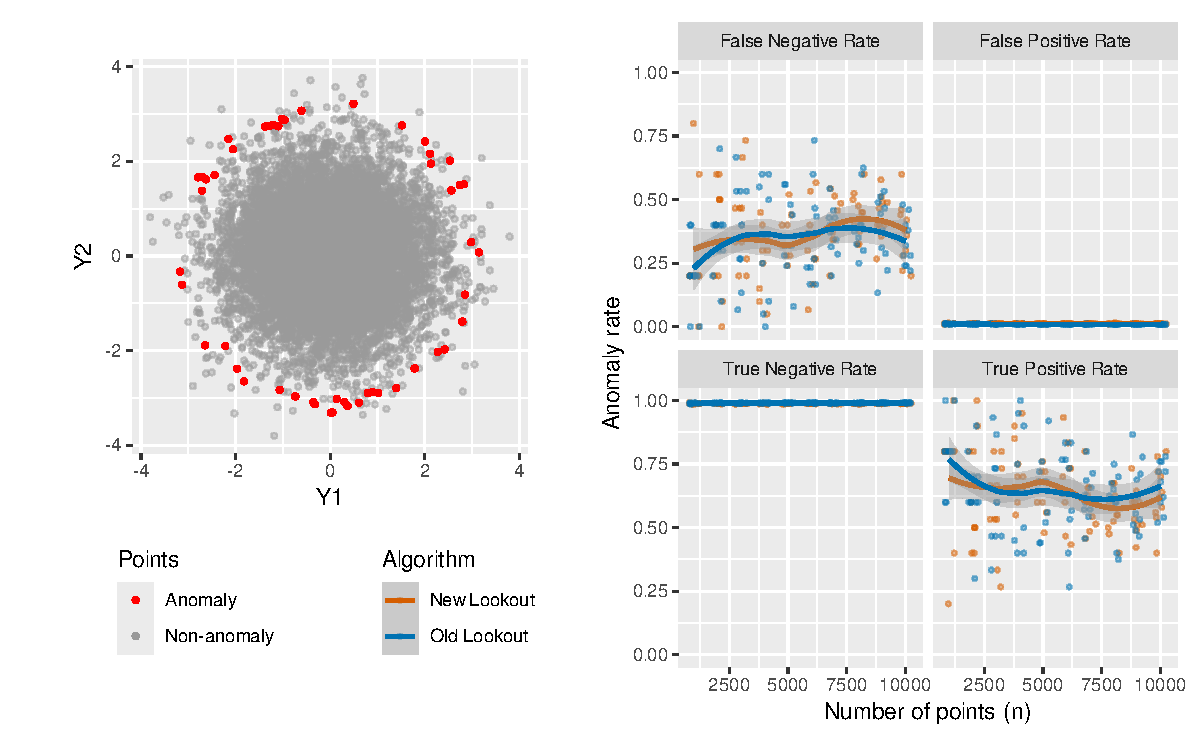
\includegraphics[width=\textwidth]{Figures/Exp2.pdf}
  \caption{Experiment 2. Left: data for $n=10000$. Right: error rates of the two versions of lookout, with points jittered horizontally.}
  \label{fig:exp2}
\end{figure}

\cref{fig:exp2} shows the data of one replication and the results. The false positive rates are about 0.012 for the new version and 0.010 for the original. The two versions have similar true positive rates at every $n$, between about 0.55 and 0.8. The online Appendix repeats this experiment with gamma-distributed observations (Experiment S2); there the two versions differ little, and the original is slightly better at the largest sample sizes.

\subsection{Experiment 3: Normal distributions moving out in each iteration}

The sample has 405 points in $\R^6$, of which five are anomalies. The non-anomalies are $\mathcal{N}(0,1)$ in every dimension. The anomalies differ from the non-anomalies only in the first dimension, where they are $\mathcal{N}(1.5 + 0.5i,\, 0.2^2)$ at iteration $i \in \{1, \ldots, 10\}$, so they move further from the non-anomalous points at each iteration. Each iteration is repeated 10 times.

\begin{figure}[!b]
  \centering
  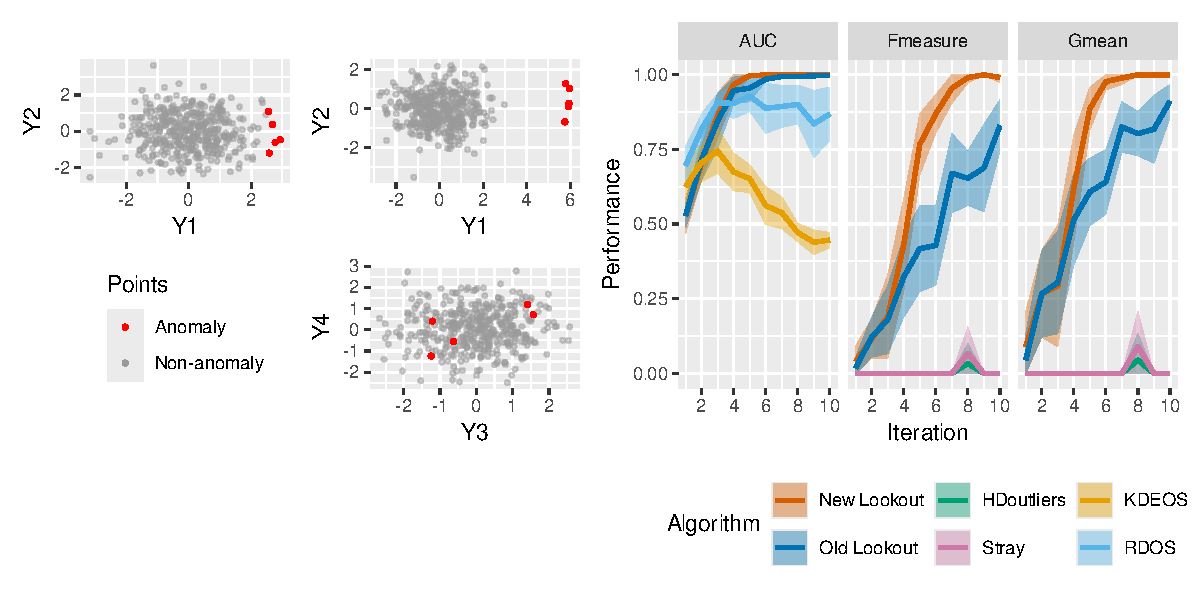
\includegraphics[width=\linewidth]{Figures/Exp3_Data_and_Results.pdf}
  \caption{Experiment 3. Left: the $Y_1Y_2$ plane at the third iteration, with anomalies in red. Middle: the $Y_1Y_2$ (top) and $Y_3Y_4$ (bottom) planes at the ninth iteration. Right: mean AUC, Fmeasure and Gmean over ten replications, with bands of $\pm2$ standard errors, for the two versions of lookout, HDoutliers, KDEOS, RDOS and stray.}
  \label{fig:exp3}
\end{figure}

\cref{fig:exp3} shows the data at the third and ninth iterations, and the results. By the ninth iteration the anomalies have separated from the other points in the $Y_1$ direction, but they remain mixed with them on the $Y_3Y_4$ plane. The new version has higher Fmeasure and Gmean than the original from the fourth iteration, and the two versions have similar AUC. RDOS has the highest AUC in the first three iterations; from the fourth, both versions of lookout are at least as good as the four other methods on every metric.

\subsection[Experiment 4: Annulus in R3]{Experiment 4: Annulus in $\R^3$}

\begin{figure}[!b]
  \centering
  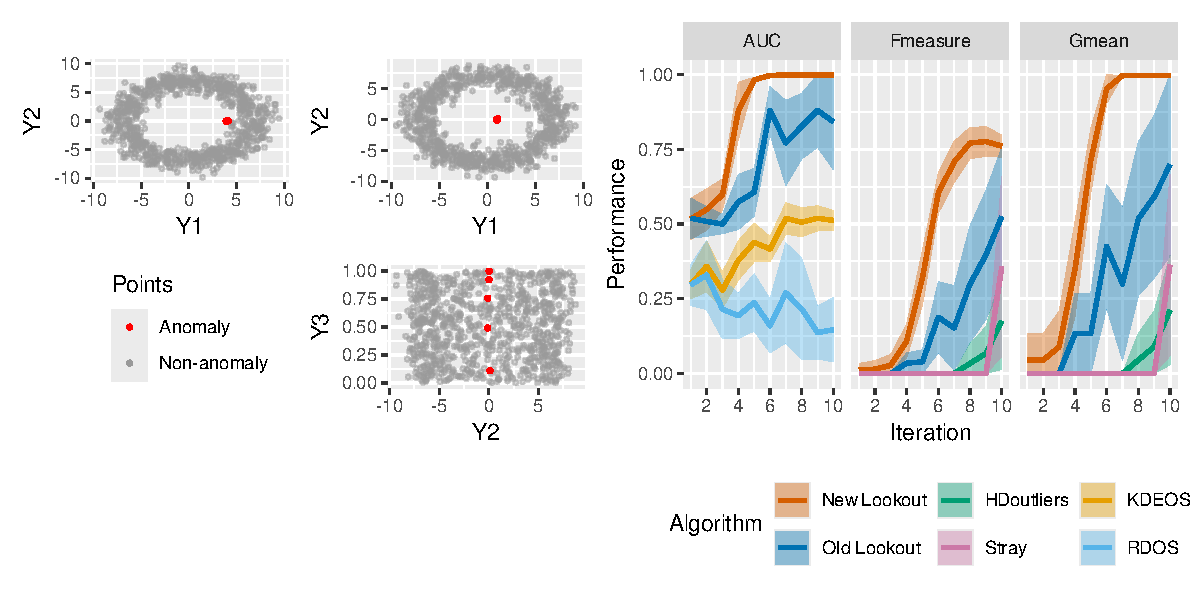
\includegraphics[width=\linewidth]{Figures/Exp4_Data_and_Results.pdf}
  \caption{Experiment 4. Left: the $Y_1Y_2$ plane at the third iteration, with anomalies in red. Middle: the $Y_1Y_2$ (top) and $Y_2Y_3$ (bottom) planes at the ninth iteration. Right: mean AUC, Fmeasure and Gmean over ten replications, with bands of $\pm2$ standard errors, for the two versions of lookout, HDoutliers, KDEOS, RDOS and stray.}
  \label{fig:exp4}
\end{figure}

The sample has 805 points in $\R^3$, of which five are anomalies. On the $Y_1Y_2$ plane the non-anomalies lie in an annulus, with uniform angle and $\mathcal{N}(7, 1)$ radius, and $Y_3 \sim \mathcal{U}(0,1)$ for all points. At iteration $i \in \{1, \ldots, 10\}$ the anomalies have $Y_1 \sim \mathcal{N}(5.5 - 0.5i,\, 0.1^2)$ and $Y_2 \sim \mathcal{N}(0, 0.1^2)$, so they move from the inner edge of the annulus towards the centre of the hole. Each iteration is repeated 10 times. \cref{fig:exp4} shows the data at iterations 3 and 9 and the results. The AUC and Gmean of the new version are close to one from the seventh iteration, when it identifies all five anomalies in every replication; its Fmeasure levels off at about 0.77 because of false positives. The original version is lower and more variable, KDEOS and RDOS have AUC of at most about 0.5 throughout, and HDoutliers and stray identify almost no anomalies before the eighth and tenth iterations respectively.

\subsection[Experiment 5: Unit cube in R20]{Experiment 5: Unit cube in $\R^{20}$}

The sample has 500 points in $\R^{20}$, of which one is an anomaly. Initially all 500 points are uniform on $(0,1)$ in each dimension. At iteration $i \in \{1, \dots, 20\}$ the first $i$ coordinates of the anomaly are set to $0.9$, so that at iteration 20 it is $(0.9, \dots, 0.9)$, and each iteration is repeated 10 times. The anomaly is not anomalous in any single coordinate, on any $Y_iY_j$ plane or in the first two principal components, so \cref{fig:exp5} shows the $D_1D_2$ plane of the projection given by \textit{dobin} \citep{dobinPaper}, a dimension reduction method designed for anomalies, at iterations 5, 12 and 20, together with the results. The anomaly is mixed with the other points at iteration 5 and separated from them at iterations 12 and 20. Both versions of lookout are run without scaling. The AUC of the new version is close to one from the twelfth iteration except at the fourteenth, and that of RDOS from about the eleventh; the original version and KDEOS are lower. The Gmean of the new version is close to one from the sixteenth iteration, when it identifies the anomaly in every replication. Its Fmeasure stays below 0.5 because of about three false positives among the 499 non-anomalies. HDoutliers and stray never identify the anomaly.

\begin{figure}[!tb]
  \centering
  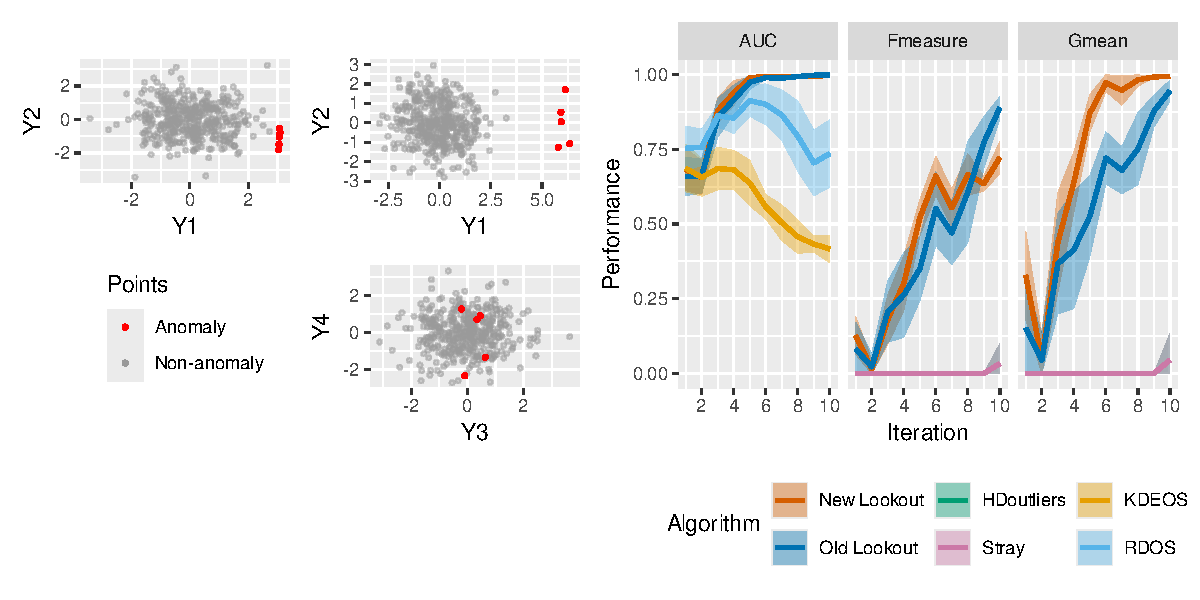
\includegraphics[width=\linewidth]{Figures/Exp5_Data_and_Results.pdf}
  \caption{Experiment 5. Left: the $D_1D_2$ plane of the dobin projection at the fifth, twelfth and twentieth iterations, with the anomaly in red. Right: mean AUC, Fmeasure and Gmean over ten replications, with bands of $\pm2$ standard errors, for the two versions of lookout, HDoutliers, KDEOS, RDOS and stray.}
  \label{fig:exp5}
\end{figure}

\subsection{Sensitivity to the bandwidth}\label{sec:bwablation}

\cref{sec:whynotmise} argues that the bandwidth should be of the order of the spacing in the tails, and that neither the constant nor MISE-optimality matters much. To check this, we repeated Experiments 1, 2 and 3, and Experiment S1 of the online Appendix, with $h_n$ multiplied by $1/4$, $1/2$, $2$ and $4$, and with $h_n$ replaced by the AMISE-optimal bandwidth $h_{\text{opt}}$ of \cref{tab:bwconst}. The details and results are in the online Appendix. The area under the ROC curve was almost the same for every bandwidth from $h_n/2$ to $4h_n$, so the ranking of the observations is insensitive to the bandwidth. The threshold is more sensitive. At $h_n$ the false positive rate was close to the nominal $\alpha=0.01$, and at $h_n/4$ it was between $0.05$ and $0.27$, because observations with no other observation inside the kernel support are all declared anomalous. With $h_{\text{opt}}$ the results were similar to those at $h_n$ for normal data in two dimensions. In six dimensions $h_{\text{opt}}$ was about a quarter of $h_n$.
